\documentclass[12pt,fleqn,leqno,letterpaper]{article}
\usepackage{lmodern}
\usepackage{relsize}
\usepackage[textwidth=7in,textheight=11in]{geometry}% http://ctan.org/pkg/geometry
\usepackage{amsmath, amsthm, amssymb, mathtools}
\usepackage{mathrsfs}

\usepackage{graphicx}
\usepackage{adjustbox}


\title{Homework 7}
\author{Alex Day\\
	\small{Analysis of Linear Systems}
}
\date{\today}

\newtheorem{theorem}{Theorem}

\newenvironment{subproof}[1][\proofname]{%
  \renewcommand{\qedsymbol}{$\blacksquare$}%
  \begin{proof}[#1]%
}{%
  \end{proof}%
}

\newcommand{\norm}[1]{\left\lVert#1\right\rVert}

\begin{document}
	\maketitle

    \begin{enumerate}
        \item[3]
            \begin{align*}
                \norm{A \circ B}_{X, Y} &:= \sup_{x \ne \bigodot_{X}} \frac{\norm{A \circ B(x)}_{Y}}{\norm{x}_{X}}\\
                &\le \sup_{x \ne \bigodot_{X}} \norm{A}_{X,Y} \frac{\norm{B(x)}_{Y}}{\norm{x}_{X}}\\
                &\le \norm{A}_{X,Y} \sup_{x \ne \bigodot_{X}}  \frac{\norm{B(x)}_{Y}}{\norm{x}_{X}}\\
                &\le \norm{A}_{X,Y} \norm{B}_{X,Y}
            \end{align*}
        \item[5a.]
            \begin{minipage}[t]{\linewidth}
                \raggedright
                \adjustbox{valign=t}{%
                    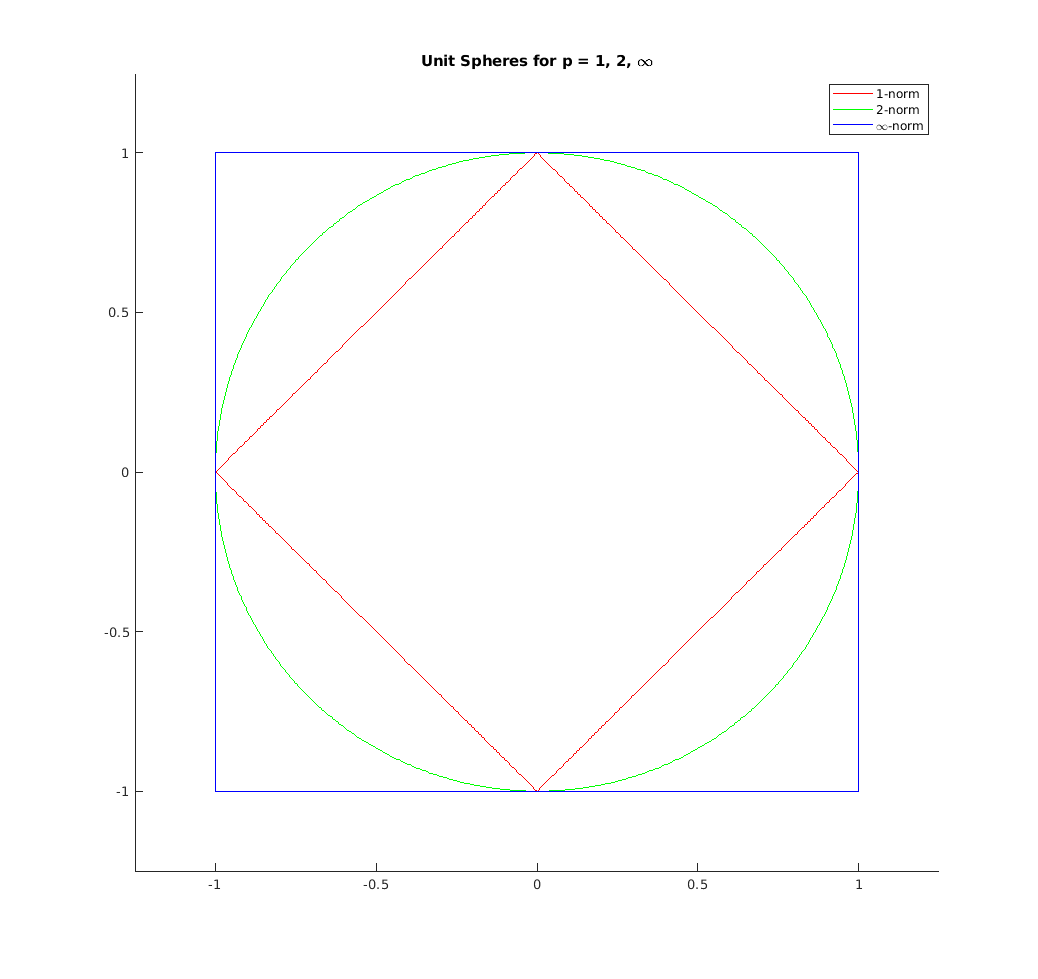
\includegraphics[width=\linewidth]{unit_sphere.png}%
                }
                \medskip
            \end{minipage}
        \item[5b.]
            \begin{align*}
                A &= \begin{bmatrix} 1 & 2 \\ 3 & 4 \end{bmatrix}\\
                    \norm{A}_{1} &= \max_{j = 1, 2} \sum_{i = 1}^{n} \lvert a_{ij} \rvert &&= 6\\
                    \norm{A}_{2} &= \max_{i = 1, 2} \sqrt{\lambda_{i} (A^{*}A)} &&=5.3723 \\
                    \norm{A}_{\infty} &= \max_{i = 1, 2} \sum_{j = 1}^{n} \lvert a_{ij} \rvert &&= 7
             \end{align*}
        \item[5c.]
            \begin{minipage}[t]{\linewidth}
                \raggedright
                \adjustbox{valign=t}{%
                    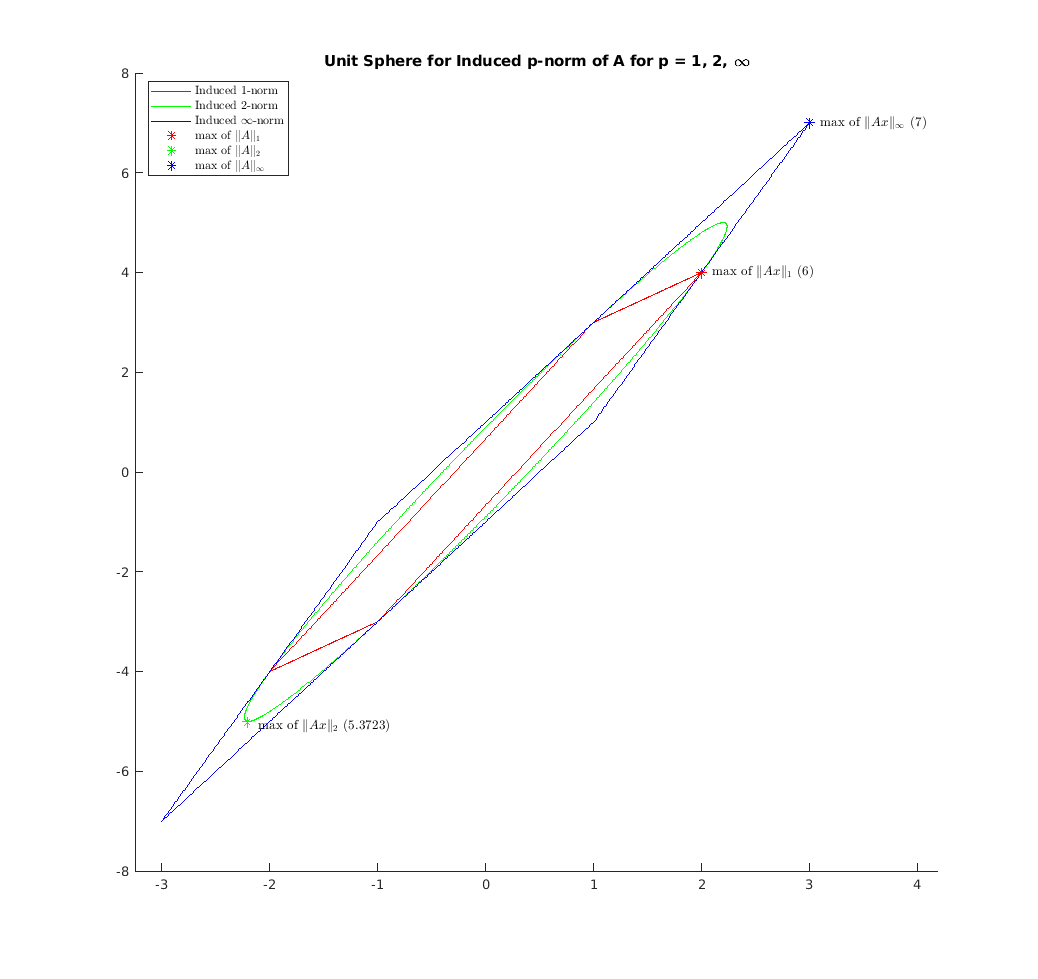
\includegraphics[width=\linewidth]{induced_unit_sphere.png}%
                }
                \medskip
            \end{minipage}
        \item[6e.]
            \begin{align*}
                A &= \begin{bmatrix}1 & 4 & 2 & 5 \\ 8 & 4 & 3 & 1\end{bmatrix}\\
                y &= Ax\\
                \norm{Ax}_{Y} &\le \alpha \norm{x}_{X}\\
                \norm{Ax}_{Y} &\le \norm{A}_{X,Y} \norm{x}_{X}\\
                \norm{Ax}_{2} &\le \norm{A}_{\infty, 2} \norm{x}_{\infty}\\\\
                \norm{A}_{\infty, 2} &:= \max_{\norm{\hat{x}_{\infty}} = 1} \norm{A\hat{x}}_{2} = 20 && \text{(calculated by brute force using MATLAB)}\\\\
                \alpha &= 20\\
            \end{align*}
	\end{enumerate}
\end{document}
























